\documentclass[12pt]{article}

\usepackage{amsmath,amsthm,xspace,multirow}
\usepackage[margin=1in]{geometry}
\usepackage{graphicx,grffile}

\usepackage{amsmath} % essential for cases environment
\usepackage{amsthm} % for theorems and proofs
\usepackage{amsfonts} % mathbb
\usepackage{marvosym}
\usepackage{xspace}
\usepackage{multirow} % fancy tables
\usepackage{wasysym} % circle symbols (including half-filled circles)
\usepackage{enumerate} % fancier enumeration (e.g., a,b,c, ...)
%\usepackage{xcolor}
\usepackage{color}
\usepackage{mathtools}
\usepackage{tikz}
\usepackage{oubraces}
\usepackage{hyperref}
\usepackage[toc,page]{appendix}
\usepackage{cleveref}
\usepackage{cite}
\usepackage{textcomp}

\usepackage{algpseudocode,algorithm}
\usepackage{caption}
%used for spacing in list of figures/tables
\usepackage{tocloft}
%predominantly used for list of abbreviations and symbols
\usepackage{longtable}
\usepackage{enumitem}
	\newlist{abbrv}{itemize}{1}
	\setlist[abbrv,1]{label=,labelwidth=1in,align=parleft,itemsep=0.1\baselineskip,leftmargin=!}

%langauge
\usepackage[english]{babel}

%Tabular Commands
\usepackage{array}
\newcolumntype{L}[1]{>{\raggedright\let\newline\\\arraybackslash\hspace{0pt}}m{#1}}
\newcolumntype{C}[1]{>{\centering\let\newline\\\arraybackslash\hspace{0pt}}m{#1}}
\newcolumntype{R}[1]{>{\raggedleft\let\newline\\\arraybackslash\hspace{0pt}}m{#1}}

%make align work with lineno

\newcommand*\patchAmsMathEnvironmentForLineno[1]{%
  \expandafter\let\csname old#1\expandafter\endcsname\csname #1\endcsname
  \expandafter\let\csname oldend#1\expandafter\endcsname\csname end#1\endcsname
  \renewenvironment{#1}%
     {\linenomath\csname old#1\endcsname}%
     {\csname oldend#1\endcsname\endlinenomath}}% 
\newcommand*\patchBothAmsMathEnvironmentsForLineno[1]{%
  \patchAmsMathEnvironmentForLineno{#1}%
  \patchAmsMathEnvironmentForLineno{#1*}}%
\AtBeginDocument{%
\patchBothAmsMathEnvironmentsForLineno{equation}%
\patchBothAmsMathEnvironmentsForLineno{align}%
\patchBothAmsMathEnvironmentsForLineno{flalign}%
\patchBothAmsMathEnvironmentsForLineno{alignat}%
\patchBothAmsMathEnvironmentsForLineno{gather}%
\patchBothAmsMathEnvironmentsForLineno{multline}%
}

%commenting commands
\newcommand{\spenny}[1]{{\color{red}{(\bfseries Spenny: }{\em #1})}}
%\renewcommand{\spenny}[1]{}

%colours

\definecolor{dodgerblue}{RGB}{30,144,255}
\definecolor{darkorchid1}{RGB}{172,29,255}
\definecolor{orange}{RGB}{255,149,0}
\definecolor{forestgreen}{RGB}{0,122,16}
\newcommand{\red}[1]{{\color{red}#1}}

\newtheorem{theorem}{Theorem}[section]
\newtheorem{lemma}{Lemma}[section]
%\renewcommand\qedsymbol{\Coffeecup}
\newcommand{\Note}[1]{\textbf{\emph{Note:}\xspace#1}}
%Greek Letter shortcuts
\newcommand{\lam}{\lambda}
\newcommand{\Lam}{\Lambda}
\newcommand{\gam}{\gamma}
\newcommand{\Gam}{\Gamma}
\newcommand{\eps}{\varepsilon}


\newcommand{\ee}{(\hat{P_1},\hat{P_2},\hat{P_{12}})}
\newcommand{\eep}{\left(1-\frac{\mu}{f_1}\right)}
\newcommand{\eef}{\left(1-\frac{\mu}{f_1},0,0\right)}
\newcommand{\JD}[1]{{\color{blue}{\bfseries Jonathan:} #1}}
\newcommand{\EEZone}{\frac{\beta}{\alpha}\left(1-\frac{\mu}{\gam}\right)}

%Simulation Commands/Macros
\newcommand{\neigh}{{\cal N}}
\newcommand{\state}{\text{state}}
\newcommand{\cmax}[1]{\ensuremath c_{\rm #1}}
\newcommand{\heal}{\text{H}}
\newcommand{\susc}{\text{S}}
\newcommand{\expose}{\text{E}}
\newcommand{\infect}{\text{I}}


%Commenting commands:
\newcommand{\Question}[1]{{\em \bf Question:} #1}
\newcommand{\Answer}[1]{{\em \bf Answer:} #1}

%Unit commands
\newcommand{\mum}{\ensuremath \mu{\rm m}}
\newcommand{\cm}{\ensuremath {\rm cm}}
\newcommand{\mm}{\ensuremath {\rm mm}}

\newcommand{\f}{f}

%Equilibrium macros
\newcommand{\HE}{\textit{HE}\xspace}
\newcommand{\DE}{\textit{DE}\xspace}
\newcommand{\equil}{(\bar{H},\bar{S},\bar{E},\bar{I},\bar{V},\bar{Z})}
\newcommand{\eq}[1]{\overline{#1}}


%% macros
\newcommand{\Reals}{\mathbb{R}}
\newcommand{\term}[1]{{\bfseries\slshape #1}}
\newcommand{\Ker}{{\text{Ker}\,}}
\newcommand{\argmax}{{\text{argmax}}}
\newcommand{\argmin}{{\text{argmin}}}
\newcommand{\Range}{{\text{Range}\,}}
\newcommand{\norm}[1]{\left\|#1\right\|}
\newcommand{\abs}[1]{\left|#1\right|}
\newcommand{\R}{{\cal R}}
\newcommand{\G}{{\cal G}}
\newcommand{\N}{{\cal N}}
\newcommand{\Tinf}{T_\textrm{inf}}
\newcommand{\Prob}{\textrm{Pr}}
\newcommand{\Shat}{{\hat{S}}}
\newcommand{\Ihat}{{\hat{I}}}
\newcommand{\ie}{\emph{i.e., }}
\newcommand{\eg}{\emph{e.g., }}
% \newcommand{\Rlogo}{\protect\includegraphics[height=2ex,keepaspectratio]{images/Rlogo.pdf}\xspace}
\newcommand{\Rlogo}{\textbf{\textsf{R}}\xspace}
\newcommand{\XPPAUT}{\texttt{XPPAUT}\xspace}
\newcommand{\etal}{\textit{et al}.\xspace}
\newcommand\emphblue[1]{\emph{\color{blue}#1}}
\newcommand{\citehere}{{\large \bf CITE HERE}}

%derivative notation
\newcommand{\D}[2]{\frac{\mathrm{d}#1}{\mathrm{d}#2}}
\newcommand{\partD}[2]{\frac{\partial \mathrm{d}#1}{\partial #2 			\mathrm{d}t}}
\newcommand{\at}[2][]{\left. #1\right|_{#2}}
\newcommand{\partd}[2]{\frac{\partial #1}{\partial #2}}
\newcommand{\x}{\text{\bf x}}
\newcommand{\Mod}[1]{\ (\text{mod}\ #1)}
%THESE ARE SPENCER'S MACROSSSSSSS

\newcommand{\A}{\frac{\alpha\delta(\rho+\chi)}{\chi\beta f}}
\newcommand{\perday}{{$\text{day}^{-1}$\xspace}}

%Text Macros
\newcommand{\TM}{\textsuperscript{TM}\xspace}

\definecolor{dkgreen}{rgb}{0,0.6,0}
\definecolor{gray}{rgb}{0.5,0.5,0.5}
\definecolor{mauve}{rgb}{0.58,0,0.82}

%-----------------
% Listings Package for code script
%-----------------
\usepackage{listings}


\lstset{ %
  language=R,                     % the language of the code
  basicstyle=\footnotesize\ttfamily,       % the size of the fonts that are used for the code
  numbers=left,                   % where to put the line-numbers
  numberstyle=\tiny\color{gray},  % the style that is used for the line-numbers
  stepnumber=1,                   % the step between two line-numbers. If it's 1, each line
                                  % will be numbered
  numbersep=5pt,                  % how far the line-numbers are from the code
  backgroundcolor=\color{white},  % choose the background color. You must add \usepackage{color}
  showspaces=false,               % show spaces adding particular underscores
  showstringspaces=false,         % underline spaces within strings
  showtabs=false,                 % show tabs within strings adding particular underscores
  frame=none,                   % adds a frame around the code
  rulecolor=\color{black},        % if not set, the frame-color may be changed on line-breaks within not-black text (e.g. commens (green here))
  tabsize=2,                      % sets default tabsize to 2 spaces
  captionpos=b,                   % sets the caption-position to bottom
  breaklines=true,                % sets automatic line breaking
  breakatwhitespace=false,        % sets if automatic breaks should only happen at whitespace
  title=\lstname,                 % show the filename of files included with \lstinputlisting;
                                  % also try caption instead of title
  keywordstyle=\color{blue},      % keyword style
  commentstyle=\color{dkgreen},   % comment style
  stringstyle=\color{mauve},      % string literal style
  escapeinside={\%*}{*)},         % if you want to add a comment within your code
  morekeywords={*,...}            % if you want to add more keywords to the set
} 



\usepackage{tikz}
\usetikzlibrary{
arrows,decorations.pathmorphing,backgrounds,positioning,fit,calc,scopes,shapes.misc
}


\tikzset{
	auto,
	compartment/.style={
		rectangle, minimum size=9mm, rounded corners=2mm,
		thick, draw=black!15, top color=white,bottom color=black!30
	},
	%
	bigcompartment/.style={
		rectangle, minimum size=24mm, rounded corners=5mm,
		thick, draw=black!15, top color=white,bottom color=black!20
	},
	%
	point/.style={
		circle, inner sep=2pt, fill=black!5
	},
	%
	mytextbox/.style={
		rectangle, text=black!50, thin, 
		draw=white, top color=white,bottom color=white, fill=white
	}
	
}

\tikzset{cross/.style={cross out, draw=black, minimum size=2*(#1-\pgflinewidth), inner sep=0pt, outer sep=0pt},
%default radius will be 1pt. 
cross/.default={5pt}}

\newcommand{\SIRboxes}
{
\node (S) [bigcompartment,bottom color=blue!30]{{S}};
\node (SI) [right=of S]{};
\node (I) [bigcompartment,right=of SI,bottom color=red!30]{I};
\node (IR) [right=of I]{};
\node (R) [bigcompartment,right=of IR,bottom color=green!30]{R};
}
\newcommand{\sirvec}[2]{ 
	\draw[->, very thick] (S) to node[midway]{#1}(I) ;
	%\node (SIparam) [above of= SI]{#1}; 
	\draw[->, very thick] (I) to node[midway]{#2}(R);
	%\node (IRparam) [above of=IR]{#2}; 
}


\newcommand{\sirs}[1]{ 
	\draw[->, very thick] (R) 
		to  [bend left=45] node[midway] {#1} (S) ;
		 
}


\newcommand{\SIboxes}
{
\node (S) [bigcompartment,bottom color=blue!30]{{S}};
\node (SI) [right=of S]{};
\node (I) [bigcompartment,right=of SI,bottom color=red!30]{I};
}

\newcommand{\sivec}[1]{ 
	\draw[->, very thick] (S) to node[midway]{#1}(I) ;
	%\node (SIparam) [above of= SI]{#1};  
}

\newcommand{\sis}[1]
{
	\draw[->, very thick] (I) 
		to  [bend left=45] node[midway] {#1} (S) ;
}

\newcommand{\SILboxes}
{
\node (S) [bigcompartment,bottom color=blue!30]{S};
\node (SI) [right= of S]{};
\node (I) [bigcompartment,right=of SI,bottom color=red!30]{I};
\node (IL) [right=of I]{};
\node (L) [bigcompartment,right=of IL,bottom color=yellow!30]{L};
}







\usepackage{tikz}
\newdimen\mylw
\tikzset{chemeq/.style={draw,thick,double distance=2pt,onearc-onearc,/chemeq/size={#1}}}
\tikzset{chemeq/.default={.4pt 6pt}}
\pgfkeys{/chemeq/size/.code={\pgfsetarrowoptions{onearc}{#1}}}
\def\parseopts#1 #2{\xdef\myalw{#1}\xdef\myasize{#2}}
\pgfarrowsdeclare{onearc}{onearc}{%
  {\edef\x{\pgfgetarrowoptions{onearc}}\expandafter\parseopts\x}
  \mylw=\myalw
  \pgfarrowsleftextend{-\myasize-.5\mylw}
  \pgfarrowsrightextend{0pt}
}{%
  \pgfsetdash{}{0pt}
  {\edef\x{\pgfgetarrowoptions{onearc}}\expandafter\parseopts\x}
  \mylw=\pgflinewidth
  \pgfsetlinewidth{\myalw}
  \pgfpathmoveto{\pgfpoint{-\myasize}{-\myasize-.5\mylw}}%
  \pgfpatharc{180}{90}{\myasize}
  \pgfusepathqstroke
}

\title{Exploring the Effects of Vaccinating Men and Including Queer Interactions in HPV Transmission Models}
\author{Spencer Hunt and Dr. Jonathan Dushoff}
\begin{document}
\maketitle

\section{Introduction}
\begin{itemize}
\item brief HPV background: virus that infects the epithelium; many different types spread sexually; associated with cervical cancer and other cancers.
\item Go into the history of vaccination: Gardasil and Cervarix, protected types, vaccination strategies in Canada (girls only)
\item Discuss some of the possible holes in this strategy: increased prevalence of oropharyngeal cancer in men with HPV, limited to no protection of queer men. 
\item Discuss some models previous results
\end{itemize}

The human papillomavirus (HPV) is a virus that infects the epithelium.  There are many types of HPV and these types are classified as high-risk or low-risk based on the association with the development of cancerous and pre-cancerous lesions.  The role of HPV infections in the development of cervical cancers has been studied extensively.  It is now know that infections with high-risk HPV types is the cause of almost all cases of cervical cancer.  However, HPV infections with these high-risk types are also associated with other cancers such as vaginal, anal, penile, and oropharyngeal cancers.  To combat the effects of HPV on cervical cancer cases, two HPV vaccines have been developed to protect against the HPV types most highly associated with pre-cancerous and cancerous lesions. Cervarix is a bivalent vaccine, which protects against HPV types -16 and -18, the two types most highly associated with cancerous development.  Gardasil is a quadravalent vaccine that protects against two low-risk HPV types -6 and -11 (most highly associated with genital warts) in addition to protecting against HPV-16 and HPV-18.  Both of these vaccines have been marketed toward girls and have been included in the routine vaccination programs for girls in many Canadian provinces and territories.  Because HPV is also highly associated with cancer in men---penile, anal, and oropharyngeal cancers---there has been a debate about whether to include boys in the routine immunization programs.  

The risk of HPV associated cancers in men has increased. In particular, the rate of oropharyngeal cancers in men has increased substantially.  This has led researchers to consider the cost-effectiveness of including boys in the routine immunization programs.  A number of studies have developed models to examine this question, and many of the results from these studies are consistent.  If vaccination rates in girls remains high, then they provide sufficient herd immunity for boys and thus can minimize the cost of administering the vaccine and reducing negative health outcomes.  However, many of these models neglect to consider the effects on queer boys and men.  Because queer men benefit very little if at all from the herd immunity effects of women, then not only these individuals may be at risk of infection with high-risk HPV types but may in fact act as a reservoir for HPV in the population overall.  

In this research study we develop three different HPV transmission models that consider different interacting populations.  In the first model, we consider groups of men and women and separate the group of men into two separate groups: queer men and straight men.  We still allow for queer interactions within the group of women, but we do not separate this group because we are concerned with the effects of including queer men in this transmission model.  Furthermore, at this point queer women are still included in current immunization program and thus receive direct protection from the vaccine. In the second model, we collapse the groups of queer and straight men into one group, still allowing for queer sexual interactions between men and between women.  The last model considers only heterosexual interactions and does not consider any queer interactions.  This technique is often employed in sexual transmission models.

After developing the models, we simulate results using parameter estimates from previous research.  We show that when only girls are vaccinated, queer men can act as a reservoir for HPV.  We also consider the case where queer men are targeted alongside women in HPV immunizations, a technique currently being initiated in British Columbia.  We show that this can reduce HPV prevalence in the population, but much more slowly than vaccinating all boys.  We also discuss some of the practical limitations to this technique.  Lastly, we show that by not including queer interactions, specifically queer interactions in men, then the positive effects of herd immunity on men may be over estimated. 

\section{Methods}
\begin{itemize}
\item Introduce the model, flow and system of ODEs
\item Discuss the various types of sexual mixing models:
	\begin{enumerate}
	\item Separate men into heterosexual and queer, considers queer interactions
	\item Include queer men and heterosexual men into one group, still consider queer interactions 
	\item Only include men and women and heterosexual interactions
	\end{enumerate}	
\end{itemize}

\subsection{The Model}
We set up a mathematical model to illustrate the transmission of HPV.  We first develop a basic underlying transmission model.  Our model considers three different infection states: susceptible $S$, infected $I$, and vaccinated $V$.  Individuals are assigned to a state based on their infection status and move through the states due to transmission, vaccination, and recovery.  We consider a variety of different groups including men, women, queer men, and heterosexual men.  We illustrate the movement through the different classes as a flow diagram in figure~\ref{fig:flowDiag}.
\begin{figure}[h!]
\begin{center}
\resizebox{0.5\textwidth}{!}{
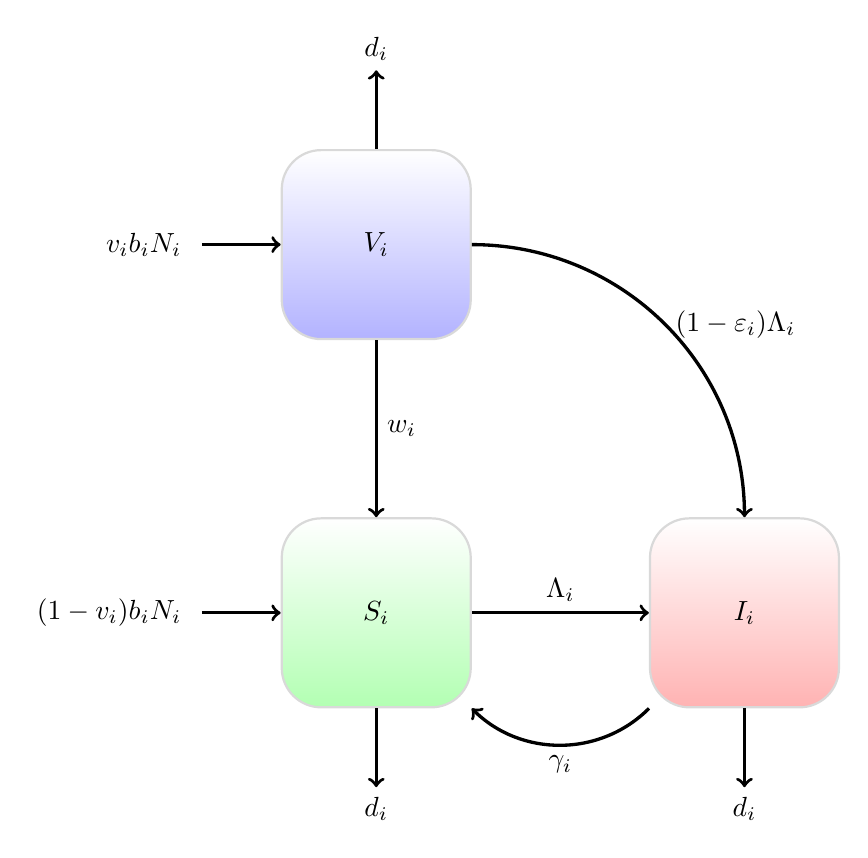
\begin{tikzpicture}
%compartments
\node (S)[bigcompartment, bottom color=green!30] {{$S_i$}};
\node (SI) [right =of S] {{}};
\node (I) [bigcompartment,right=of SI, bottom color=red!30] {{$I_i$}};
\node (SV) [above = of S] {{}};
\node (V) [bigcompartment,above=of SV, bottom color=blue!30] {{$V_i$}};

\node (leftS) [left=of S] {{}};
\node (leftV) [left=of V] {{}};
\node (downI) [below=of I] {{}};
\node (downS) [below=of S] {{}};
\node (upV) [above=of V] {{}};

%arrows
\draw[->,very thick] (S) to node[above] {$\Lambda_i$} (I);
\draw[->,very thick] (leftS) node[left] {$(1-v_i)b_iN_i$}  to (S);
\draw[->,very thick] (leftV) node[left] {$v_ib_iN_i$} to (V);
\draw[->,very thick] (V) to node[right] {$w_i$} (S);

\draw[->,very thick] (I) to[bend left=45] node[below] {$\gamma_i$} (S);
\draw[->, very thick] (V) to[bend left=45] node[right] {$(1-\eps_i)\Lambda_i$} (I);
\draw[->, very thick] (V) to (upV) node[yshift=1ex] {$d_i$};
\draw[->, very thick] (S) to (downS) node[yshift=-1ex] {$d_i$};
\draw[->, very thick] (I) to (downI) node[yshift=-1ex] {$d_i$};

\end{tikzpicture}
}
\caption{Flow diagram of the HPV transmission model.}
\label{fig:flowDiag}
\end{center}
\end{figure}
The biological parameters $\Lambda_i$ and $\gamma_i$ represent the force of transmission for individuals and the recovery from HPV in group $i$, respectively.  We consider an SIS model here because natural infection with HPV does not prevent reinfection with the same type.  Vital parameters $b_i$ and $d_i$ represent the birth and death rates, respectively.  To simplify our model we consider a constant population and set $b_i=d_i$ for all groups $i$.  The population size of group $i$ is $N_i=S_i+I_i+V_i$.  We also consider various vaccination parameters.  The value of $v_i$ is the proportion of the population that is vaccinated entering the system.  The parameter $w_i$ represents the rate at which vaccination wanes.  Because the HPV vaccines are relatively new, it is not quite clear for how long they provide protection.  Therefore, $1/w_i$ is the average time that the vaccine provides protection.  Lastly, the parameter $\eps_i$ is the protective effects of the vaccine. This values ranges from 0 (no protection) to 1 (complete protection).  This model can also be represented as a system of differential equations below:
\begin{subequations}
\begin{align}
\dot{S_i} &= (1-v_i)b_iN_i + w_iV_i - \Lambda_iS_i + \gamma_i I_i - d_iS_i,\\
\dot{V_i} &= v_ib_iN_i - w_iV_i - (1-\eps_i)\Lambda_iV_i  - d_iV_i,\\
\dot{I_i} &=  \Lambda_i(S_i+(1-\eps_i)V_i) - \gamma_i I_i - d_iI_i.\end{align}
\end{subequations}


\subsection{Sexual Mixing}

In our paper, we set up three different scenarios for considering sexual mixing. In the first scenario, we separate the men group into straight men $h$ and queer men $q$. The straight men have sex with women $w$ and queer men have sex with both other queer men and women.  We include queer women in the same group as straight women. Because vaccination strategies already target women, queer women benefit the greatest from the current vaccination strategies.  For this reason, we do not disentangle sexual interactions of queer women from straight women.  This scenario considers same-sex interactions and also actively tracts the infection of queer men.  We set up a sexual mixing scenario where group $i$ mixes with $j$ at a rate $m_{ij}$ defined as such
\begin{equation}
m_{ij} = n_ic_i p_{ij}
\end{equation}
where $n_i$ is the proportion of individuals in group $i$, $c_i$ is the contact rate for group $i$, and $p_{ij}$ is the probability of an individual in group $i$ mixing with an individual in group $j$.  We observe two restrictions in this model.  The first being symmetry as an individual in group $i$ mixes with individual in group $j$ at the same rate as an individual in group $j$ with someone in group $i$. That is
\begin{equation}
m_{ij}=m_{ji}.
\end{equation}
The second restriction is that the sum of all mixing probabilities for group $i$ must equal 1
\begin{equation}
\sum_j p_{ij} = 1.
\end{equation}
To simplify this problem, we set $r_{ij}=c_ip_{ij}$ as the effective contact rate of an individual in group $i$ with an individual in group $j$.  Thus we have that 
\begin{equation}
\sum_j r_{ij} = c_i.
\end{equation}

\subsubsection{Case 1: Queer and Straight Men Separated}

In the first case, where we track the interactions of queer men separately from straight men, we have three different groups: heterosexual men $h$, queer men $q$, and women $w$.  We set the proportion of men and women to be the same $n_m=n_w=0.5$, and set the proportion of queer men to 20\% of all men.  Considering a basic example we set $n_w=0.5$ and $n_m=0.5$.  The proportion of men who are queer is 20\% and thus $n_q=0.1$ and $n_h=0.4$.  Solve for the following mixing matrix:
\spenny{I don't think we'll actually include these basic calculations in the real paper, but I just wrote it here so it's more clear what I did to solve them.}
\begin{equation}
M = \left[\begin{array}{c c c}
0 & 0 & 1 \\
0 & 0.8 & 0.075 \\
1 & 0.075 & 0.0625 
\end{array}\right]
\end{equation}
where heterosexual men is the first row/column, queer men is the second, and women is the third.  We solve for the contact rates $c_h=2.5$, $c_q=8.75$, and $c_w=2.275$.  

\subsection{Scenario 2 - Queer and Straight Men Collapsed}
The second scenario still considers same-sex interactions, but queer men and straight men are contained within the same group, just referred to as men $m$.  Thus we have that the mixing rate between men and men comes solely from the queer men interactions:
\begin{equation}
m_{mm} = m_{qq} = 0.8
\end{equation}
and thus the effective contact rate of a man with another man is $r_{mm} = \dfrac{n_q}{n_m} r_{qq} = 8(0.2) = 1.6$.  The mixing rate of men with women come from both the straight men and the queer men. 
\begin{equation}
m_{mw} = m_{hw} + m_{qw}
\end{equation}
and thus the effective contact rate of a man with a women is $r_{mw} = \frac{n_h}{n_m}r_{hw} + \frac{n_q}{n_m}r_{rq} = 0.8(2.5)+0.2(0.75) = 2.15$.  Therefore, the over all contact rate for men is $c_m=3.75$.  This gives the final mixing matrix in this case
\begin{equation}
M = \left[\begin{array}{c c}
0.8 & 1.075 \\
1.075 & 0.0625 
\end{array}\right]
\end{equation}
where the first row/column refers to men and the second refers to women.  

\subsection{Scenario 3 - No Queer Interactions}
The last scenario only considers two groups, men and women, and only considers opposite-sex interactions.  Many HPV models up to this point only consider opposite-sex interactions, and this scenario in our paper is used to parallel the results to previous work.  Both groups of men and women here include queer and straight men and women, but we only consider opposite-sex interactions in the transmission of HPV. And thus the mixing matrix in this case only considers the opposite-sex mixing rates.  And thus the mixing matrix for this scenario is just:
\begin{equation}
M=\left[\begin{array}{c c}
0 & 1.075 \\
1.075 & 0
\end{array}\right]
\end{equation}
\section{Results}
\begin{itemize}
\item Discuss main results for each scenario of mixing and various vaccine coverage scenarios
\item Show pictures
\end{itemize}

In the first scenario, we consider men and women, separating the group of men into two groups, straight and queer men.  Queer men may have sex with both women and other queer men, straight men have sex with women exclusively.  Because women are already scheduled to take the HPV vaccine and to simplify our model, we do not separate the group of women into straight and queer women. Instead the group of women can interact with both straight and queer men, and other women. We run this system to equilibrium without any vaccine program to provide baseline infection estimates.  This is visualized in Figure \ref{fig:QueerNoVacc}.  Here we see that the number of infected women (red line) is approximately 200,000 individuals, the number of infected straight men (blue line) is approximately 160,000 individuals, and the number of infected queer men (magenta line) is approximately 20,000 individuals.  

\begin{figure}[h!]
\begin{center}
\includegraphics[width=0.8\textwidth]{base.queer.gPlot.Rout-0.pdf}
\caption{This is the equilibrium for the model that considers queer interactions in men and women, but separates the queer men out as a separate group.}
\label{fig:QueerNoVacc}
\end{center}
\end{figure}

When we introduce vaccination strategies into these populations we see some interesting trends.  The first strategy considers vaccinating women and girls exclusively.  The first scenario considers 50\% vaccine coverage in women.  When we introduce this vaccine strategy (vertical, dotted grey line) we see a reduction in HPV cases in all groups, and significant reductions in women and straight men.  This is because as more women become vaccinated, they provide herd immunity for men.  This has been documented and discussed significantly in the area of HPV vaccination research.  We observe a decrease in the prevalence of HPV in the queer men.  Again, vaccinating women provides some herd immunity to the queer men during sexual intercourse between these queer men and women.  Because queer men predominately have sexual interactions with other queer men, they do not benefit completely from the vaccination of women exclusively.  More importantly, it seems that queer men have the potential to sustain HPV given this vaccination strategy.

\begin{figure}
\begin{center}
\includegraphics[width=0.8\textwidth]{base.queer.gPlot.Rout-1.pdf}
\caption{This scenario considers queer interactions between men and women, but separates the male group into straight and queer men.  Here we apply a fully effective vaccine program covering 50\% of women exclusively}
\label{queerVaccWomen50}
\end{center}
\end{figure}

We also consider a vaccination scenario where queer men are also vaccinated alongside women (Figure~\ref{fig:QueerVaccQueer10}.  British Columbia has recently revised its HPV vaccination strategy, including queer and questioning boys and other high-risk boys in the HPV vaccination group.  We reduce the effective coverage from 50\% in girls to 10\% in queer men because of an increased risk of missing individuals.  During the time of vaccination many queer boys may not feel comfortable coming forth or may not have come to terms with their queer identity.  As such, there is likely to be a reduced vaccine coverage rate in this group.

Running the model under this scenario we see a reduction in HPV in women, straight men, and queer men.  This decline is fairly slow and may take up to over 75 years to be eliminated in the population.  

\begin{figure}[h!]
\begin{center}
\includegraphics[width=0.8\textwidth]{base.queer.gPlot.Rout-2.pdf}
\caption{In the case where we have queer interactions and queer men as a separate group, we also consider 50\% vaccination in girls and 10\% vaccination in queer boys only.  This to represent the targeted vaccine strategies including at-risk boys, but also considers limited uptake in this at-risk group.}
\label{fig:queerVaccQueer10}
\end{center}
\end{figure}

When we target vaccination to all children, boys and girls, we can assume all groups have a 50\% vaccination rate.  Because queer boys are not being isolated for vaccination, there are no social stigmas to opting into vaccination, and thus we can assume similar vaccination rates between queer and straight boys.  In this scenario all groups receive direct protection from HPV and we see as sharp decline in the prevalence, with clearance occurring early twice as soon in the case where we just vaccinate girls and queer boys.  This is visualized in Figure~\ref{queerVaccAll}

\begin{figure}[h!]
\begin{center}
\includegraphics[width=0.8\textwidth]{base.queer.gPlot.Rout-3.pdf}
\caption{Considering the case where we have queer interactions and queer men as a separate group, we induce 50\% vaccination in girls and boys.}
\label{queerVaccAll}
\end{center}
\end{figure}

\subsubsection{Queer Men and Straight Men Collapsed}

In this series of models we collapse the group of straight and queer men into one group, which we refer to as just men.  When calculating the contact rates of the group of men with women and other men, we take the weighted average of the contact rates from the separated straight and queer men groups.  

Running the base model with no vaccination (Figure~\ref{fig:menNoVacc}) we observe a significantly higher prevalence of HPV in both men and women when compared to the previous model that separated the queer and straight men into different groups.  A possibility for this phenomenon could be that by collapsing the group of queer men with other straight men, we have increased the overall contact rate between men.  In the previous case, most queer men were having sex with each other, and these individuals were contacting each other.  By expanding the group, there are more opportunities for queer interactions between more men, and this could increase the overall spread of the infection.  One possible way to address this could be to implement a sort of heterogeneity, where net queer interactions occurred less often in the collapsed group of men due double counting interactions between similar individuals.

When we introduce a vaccination strategy where only girls are vaccinated at a coverage rate of 50\%, we observe a significant decrease in the prevalence of HPV in both men and women (dashed line, Figure~\ref{fig:menGirlVacc50}).  However, we see that the infection is sustained.  This is because men are not directly protected from HPV, and thus they are able to proliferate the infection within the group of males through homosexual interactions, which also sustains the infection in women from heterosexual interactions.  Because of this, heard immunity from women exclusively is not able to eliminate HPV from the population. 

When expanding the vaccination strategy to both men and women, again at 50\% coverage for both groups, we observe a sharper decline in HPV prevalence (dashed line, Figure~\ref{fig:menAllVacc50}).  This decline is more pronounced under this strategy than when women were solely vaccinated.  Clearance is obtained under this vaccination strategy.  

\begin{figure}[h!]
\begin{center}
\includegraphics[width=0.8\textwidth]{base.men.gPlot.Rout-0.pdf}
\caption{In this scenario, we collapse queer and straight men into one group.  We run the model with no immunization strategy to obtain baseline HPV prevalence values for both boys (blue) and girls (red).}
\label{fig:menNoVacc}
\end{center}
\end{figure}
%------------------------------------
\begin{figure}[h!]
\begin{center}
\includegraphics[width=0.8\textwidth]{base.men.gPlot.Rout-1.pdf}
\caption{This scenario also considers one group of men, but introduces a vaccination strategy where girls are vaccinated at an effective coverage of 50\% (dashed lines).  In this scenario, we see a sharp decline in the prevalence of HPV, but it is sustained.}
\label{fig:menGirlVacc50}
\end{center}
\end{figure}

\begin{figure}[h!]
\begin{center}
\includegraphics[width=0.8\textwidth]{base.men.gPlot.Rout-3.pdf}
\caption{We again consider the scenario with queer and straight men combined into one group, but we expand the vaccination strategy to both girls and boys (effective coverage of 50\%).  Here we see a sharp decline in prevalence and eventual clearance of HPV (dashed lines).}
\label{fig:menAllVacc50}
\end{center}
\end{figure}




%------------------------------------------------
\newpage
\subsubsection{Scenario 3 - No Queer Men}

In this scenario, we do not consider any queer interactions.  We only consider straight men and women.  Thus the contact rates between men and between women are set to zero, $c_{mm} = c_{ww} = 0$.  Below are the baseline HPV prevalence results and the effects of a variety of vaccination strategies of this model. 

When we do not consider a vaccination strategy, we obtain baseline HPV prevalences similar to that in the first scenario, where queer men and straight men were separated in different groups (Figure~\ref{fig:noQueerNoVacc}).  When we introduce a vaccination strategy where only girls are vaccinated with 50\% coverage, we observe a sharp decline in the prevalence of HPV in both girls and boys (dashed lines, Figure~\ref{fig:noQueerGirlVacc50}).  This sharp decline in the number of infected individuals is due primarily to heard immunity.  Because a large proportion of women are protected from HPV due to vaccination, HPV cannot spread from men to these women, and then back into other men.  This eventually prevents HPV from spreading in the population, and it eventually dies out. 

By expanding the vaccination strategy to both girls and boys with an effective coverage of 50\%, we observe an even sharper decline in HPV prevalence.  The pathogen cannot spread as effectively as both men and women are protected from HPV and dies off quickly (dashed line, Figure~\ref{fig:noQueerAllVacc50}).

\begin{figure}[h!]
\begin{center}
\includegraphics[width=0.8\textwidth]{base.noQueer.gPlot.Rout-0.pdf}
\caption{In this scenario, we only consider heterosexual interactions between straight men and women.  Here we do not consider an immunization strategy and obtain baseline measures of HPV prevalence in both boys (blue) and girls (red).}
\label{fig:noQueerNoVacc}
\end{center}
\end{figure}

%------------------------------------
\begin{figure}[h!]
\begin{center}
\includegraphics[width=0.8\textwidth]{base.noQueer.gPlot.Rout-1.pdf}
\caption{This scenario only considers straight men and women, and implements a vaccination strategy where only girls are vaccinated at a effective coverage rate of 50\%.  Here we see that the prevalence of HPV in both boys and girls declines sharply and ultimately is cleared.}
\label{fig:noQueerGirlVacc50}
\end{center}
\end{figure}

\begin{figure}[h!]
\begin{center}
\includegraphics[width=0.8\textwidth]{base.noQueer.gPlot.Rout-3.pdf}
\caption{This scenario only considers straight men and women, and implements a vaccination strategy where both girls and boys are vaccinated at a effective coverage rate of 50\%.  Here we see that the prevalence of HPV in both boys and girls declines sharply (more quickly than when only vaccinating girls) and ultimately is cleared.}
\label{fig:noQueerAllVacc50}
\end{center}
\end{figure}





\section{Discussion}

In this report, we observe the effects of various vaccination strategies on three different HPV transmission models.  These models focus on the effects of homosexual interactions of queer men and women on the dynamics of HPV transmission.  We consider three different models that take into account these queer interactions.  The first model separates the group of men into queer and straight men.  Queer men can have sexual interactions with both other queer men and women, while straight men only have interactions with women.  We consider queer interactions in women as well.  Because we are concerned with how male-male sexual interactions affect disease dynamics of HPV transmission, we do no separate the group of women into two separate groups.  

Under this scenario, we observed that vaccination strategies that only target women still result in HPV infections being sustained in the population.  This is because queer men are able to act as reservoir for HPV as they only benefit minimally from the heard immunity induced by vaccinating only women.  We are able to obtain clearance of HPV when queer boys are targeted alongside girls in vaccination strategies, but clearance is slow when compared to vaccinating all three groups.  Furthermore, vaccination in exclusively queer men presents some issues surrounding access to health care and confidentiality.  If vaccination strategies require boys to opt in if they are at-risk for HPV (queer or questioning) then they may be required to disclose their sexuality before they are ready or before they come to terms with it.  Thus, vaccine coverage in this group is likely to be low, putting these boys at risk for future HPV infections.  

When we expand the HPV vaccination strategy to all three groups, we observe clearance at a much faster rate.  This is because while vaccinating solely girls can provide some herd immunity effects for those who have sex with women, vaccinating boys as well provides herd immunity for all groups.  

The second scenario we consider is where queer interactions are permitted in both men and women, but the groups of queer men and straight men are collapsed into one group.  Under this scenario and using the same contact parameters as the previous model, we observe a significant increase in HPV prevalence.  This is likely due to the increase in the number of queer interactions in the larger group of men.  As HPV spreads within the group of men due to the increase in queer interactions amongst all men, HPV also spreads into group of women through heterosexual interactions.  To correct for this, the contact rates must be changed, or the majority of queer interactions could be restricted to a smaller proportion of the group of men. 

When we implement the girls only vaccination strategy at 50\% coverage, we observe a decline in the HPV prevalence in both men and women.  However, the infection is sustained.  This is because men act as a reservoir for HPV due to the proliferation of HPV within their group through homosexual interactions.  When we expand the vaccine strategy to both boys and girls, the prevalence of HPV decreases significantly clearance is obtained. 

Lastly we consider the scenario where all queer interactions are ignored, a common technique in modelling sexually transmitted infections such as HPV.  Under this scenario, we observe a sharp decrease in HPV prevalence and clearance when we vaccinate only girls at 50\% coverage.  This is because men are not able to act as effectively as a reservoir because queer interactions are ignored.  

Previous cost-effectiveness analyses that consider only heterosexual interactions may be overestimating the effects of herd immunity when vaccinating only women.  Thus girls only immunization programs may not be as cost-effective as previously thought.  Moreover, the at-risk group of queer men may will not benefit from a girls only vaccination strategy.  






\end{document}